\documentclass{article}
\usepackage[italian]{babel}
\usepackage[tmargin=2cm,rmargin=1.5in,lmargin=1.5in,margin=0.85in,bmargin=2cm,footskip=.2in]{geometry}
\usepackage{siunitx}
\sisetup{separate-uncertainty=true, per-mode=fraction, parse-numbers=true}
\usepackage{caption}
\usepackage[T1]{fontenc}
\usepackage{bookmark}
\usepackage{mathcomp}
\usepackage{graphicx}
\usepackage{multicol}
\usepackage{booktabs}
\usepackage{amsmath,amsfonts,amsthm,amssymb,mathtools}
\hypersetup{
	pdftitle={Relazione sul pendolo quadrifilare},
	colorlinks=true, linkcolor=doc!90,
	bookmarksnumbered=true,
	bookmarksopen=true
}
\usepackage{blindtext}
\usepackage{wrapfig}
\usepackage{listings}
\usepackage{xcolor}
\usepackage{float}
\usepackage{tikz}
\usepackage{multirow}
\usepackage{biblatex}
\definecolor{codegreen}{rgb}{0,0.6,0}
\definecolor{codegray}{rgb}{0.5,0.5,0.5}
\definecolor{codepurple}{rgb}{0.58,0,0.82}
\definecolor{backcolour}{rgb}{0.95,0.95,0.92}
\definecolor{doc}{rgb}{0,0,0}
\lstdefinestyle{code}{
    backgroundcolor=\color{backcolour},   
    commentstyle=\color{codegreen},
    keywordstyle=\color{magenta},
    numberstyle=\tiny\color{codegray},
    stringstyle=\color{codepurple},
    basicstyle=\ttfamily\footnotesize,
    breakatwhitespace=false,         
    breaklines=true,                 
    captionpos=b,                    
    keepspaces=true,                                     
    showspaces=false,                
    showstringspaces=false,
    showtabs=false,                  
    tabsize=2,
    inputencoding=ansinew,
    extendedchars=true,
    numbers=left,                    
    numbersep=5pt
}

\lstset{style=code}
\usepackage[varbb]{newpxmath}
\usepackage{circuitikz}
\captionsetup{labelfont={bf, sc}}
\title{Relazione sul pendolo quadrifilare}
\author{Francesco Sermi}
\date{\today}
\begin{document}
	\maketitle
	\newpage
	\tableofcontents
	\newpage
	\section{Scopo}
		Stabilire la dipendenza che sussiste fra il periodo dell'oscillazione e la sua ampiezza
	\section{Cenni teorici}
	Il pendolo fisico (o il pendolo semplice, che può essere visto come caso particolare del pendolo fisico) può essere schematizzato nella seguente maniera:
	\begin{figure}[htbp]
		\centering
  		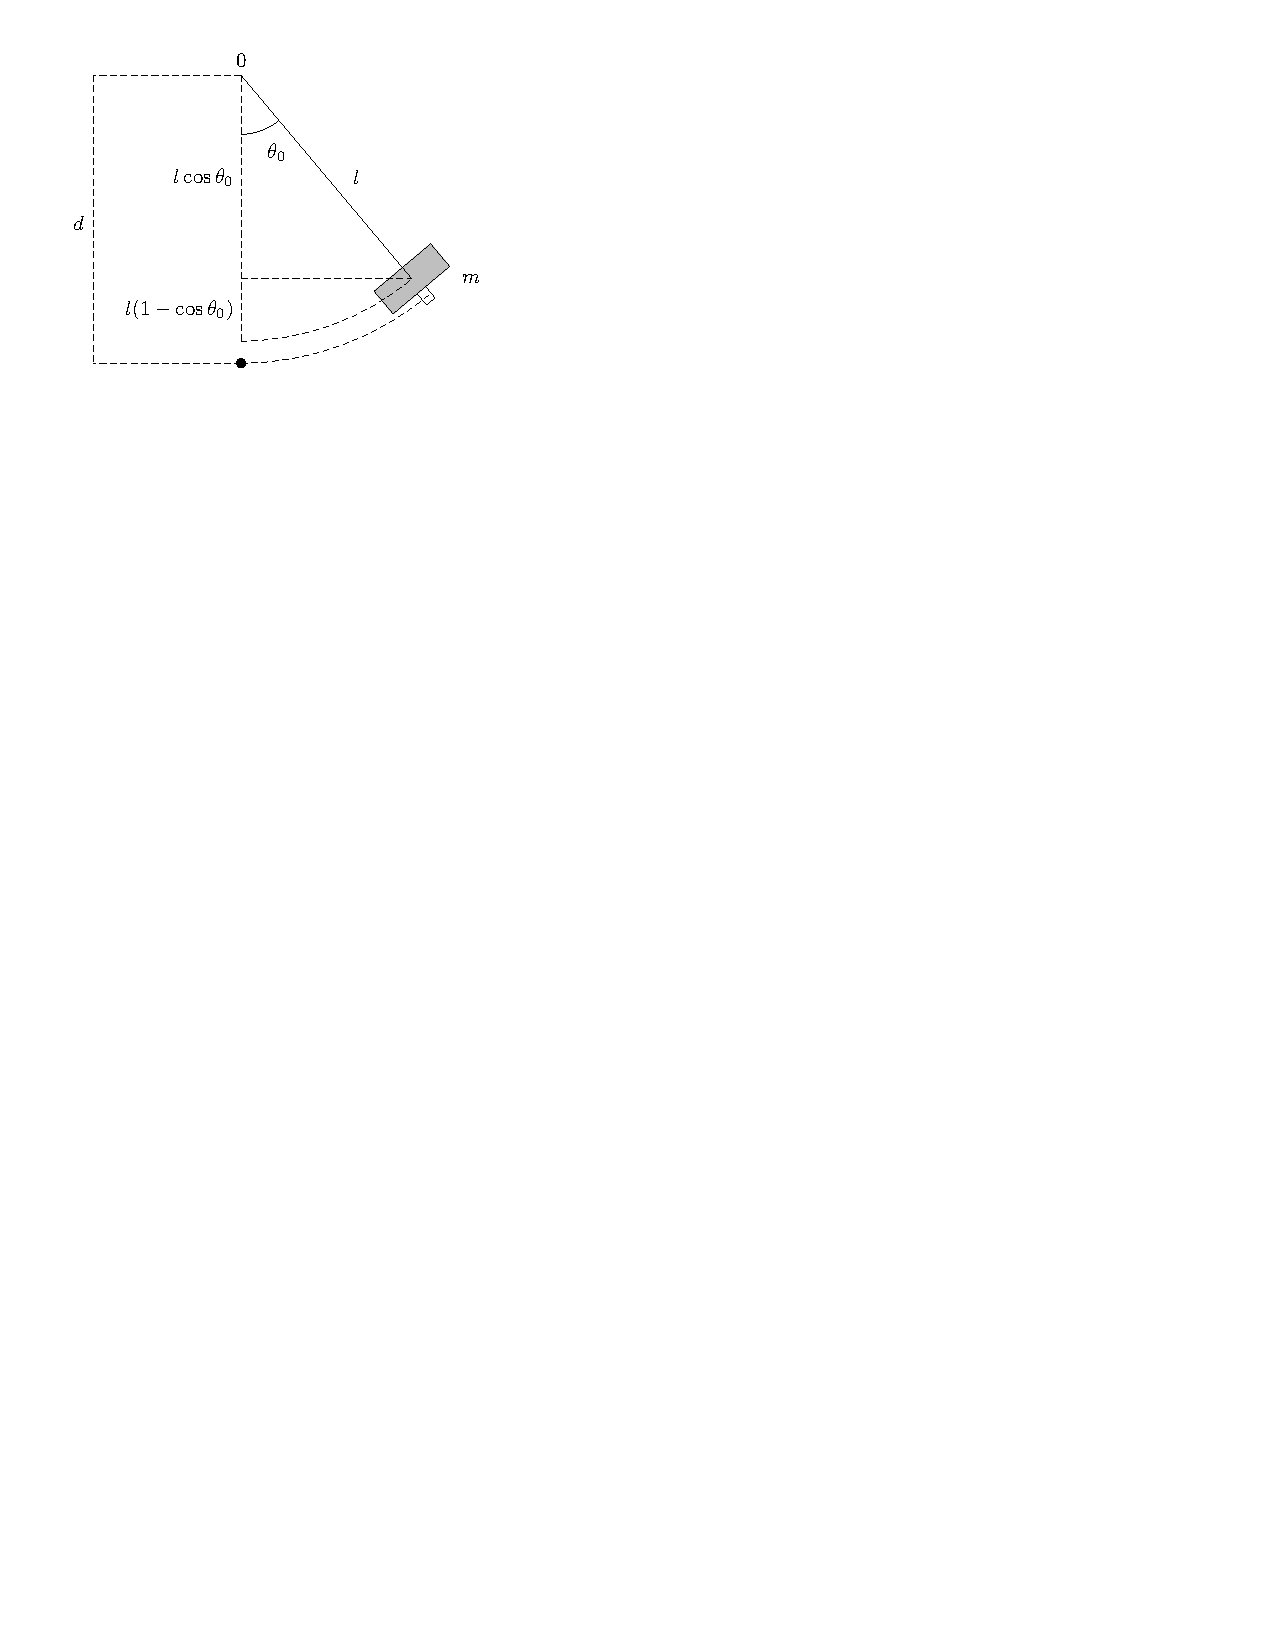
\includegraphics[scale=0.70]{pendolo_fisico_2.pdf}
  		\caption{Pendolo fisico con corpo qualunque.}
  		\label{fig:pendolo}
	\end{figure}
	Abbiamo la forza peso che induce un momento torcente rispetto al perno $O$ e la reazione vincolare $R$ che agiscono sulla massa $m$, da cui si ricava utilizzando la $II^a$ cardinale:
	\begin{equation}
		\frac{d\vec{L}}{dt} = I\ddot{\theta} = -mgl\sin{\theta}
	\end{equation}
	da cui, utilizzando l'ipotesi delle piccole oscillazioni e considerando l'espansione in serie di Taylor della funzione $\sin{(x)} = \sum\limits_{n=0}^{+\infty} \frac{(-1)^n}{(2n+1)!} x^{2n+1}$, possiamo ricondurlo all'equazione di un oscillatore armonico:
	\begin{equation*}
		I\ddot{\theta} = -mgl\theta \implies \ddot\theta = -\frac{mgL}{I}\theta
	\end{equation*}
	Da cui si ricava che, ponendo $-\omega^2 = -\frac{mgL}{I}$, che il periodo di oscillazione è pari a
	\begin{equation*}
		T = 2\pi \sqrt{\frac{I}{mgL}}
	\end{equation*}
	da cui si vede che il periodo di oscillazione non dipende, nell'ipotesi delle piccole oscillazioni, dall'angolo di oscillazione iniziale $\theta_0$. \\	
	Se non ipotizziamo le piccole oscillazioni, si può dimostrare che
	\begin{equation*}
		T = T_0 \left( 1 + \frac{1}{16}\theta_0^2 + \frac{11}{3072}\theta_0^4 + \cdots \right)
	\end{equation*}
	dove $T_0 = 2\pi\sqrt{\frac{l}{g}}$
	Ragionando in termini energetici, si osserva che l'energia meccanica si conserva nel moto (supponendo che non ci siano attriti) del pendolo e si ha che
	\begin{flalign*}
			&E_0 = mg(l-l\cos{\theta}) & \\
			& 						   & \implies \theta_0 = \arccos{ \left(1 - \frac{v_0^2}{2gL} \right) } \\
			&E_0 = \frac{1}{2}mv_0^2   & \\
	\end{flalign*}
	\section{Strumenti e materiali}
	\textbf{Materiali}:
	\begin{itemize}
		\item Pendolo quadrifilare;
	\end{itemize}
	\textbf{Strumenti}:
	\begin{itemize}
		\item Computer con programma di acquisizione;
		\item Metro a nastro, con sensibilità pari a $\pm 0.001 \si{m}$
		\item Calibro ventesimale, con sensibilità pari a $\pm 0.005 \si{\centi\meter}$
	\end{itemize}
	\section{Descrizione delle misure}
	Per effettuare questo esperimento era necessario misurare la velocità del pendolo quando incontrava la verticale, ovvero quando $\theta = 0$. Il programma di acquisizione utilizza poi la formula
\begin{align*}
	&L = (1.15 \pm 0.01) \, \si{\meter}
	&d = (1.18 \pm 0.01) \, \si{\meter}
	&w = (2.05 \pm 0.05) \, \si{\centi\meter}
\end{align*}
\end{document}